\subsection{Linked Data Indexing of Distributed Ledgers}
\label{subsec:linked-data-indexing-distributed-ledgers}

Penelitian yang dilakukan oleh \cite{third2017linked} membahas tantangan dalam pencarian informasi pada \textit{distributed ledger}, yang sulit dilakukan karena informasi mengenai suatu entitas dapat tersebar di seluruh \textit{ledger} tanpa adanya indeks. Penelitian ini mengusulkan penggunaan indeks berbasis semantik untuk Ethereum Blockchain dengan pendekatan \textit{Linked Data}, yang memungkinkan pencarian menggunakan istilah khusus sesuai \textit{domain}. Pendekatan ini diharapkan dapat meningkatkan kekuatan, kegunaan, dan cakupan dari sistem \textit{ledger} tersebut.

Dalam penelitian ini, mereka mengimplementasikan indeks semantik pada Ethereum Blockchain untuk mengekspos data di dalam \textit{distributed ledger} sebagai \textit{Linked Data}. Indeks ini mengindeks data pada level blok dan transaksi menggunakan ontologi BLONDiE, serta memetakan Smart Contract ke dalam ontologi \textit{Minimal Service Model} (MSM) sebagai langkah awal untuk menghubungkan Smart Contract dengan \textit{Semantic Web Services}.

Implementasi indeks semantik ini menggunakan ontologi BLONDiE sebagai kerangka untuk mengelompokkan dan mendeskripsikan elemen-elemen utama dari Blockchain. Ontologi \textit{Minimal Service Model}, yang biasanya digunakan untuk \textit{web services}, diterapkan untuk menggambarkan fungsionalitas dari Smart Contract pada Blockchain, sehingga memungkinkan integrasi yang lebih efisien.

\begin{figure}[ht]
  \centering
  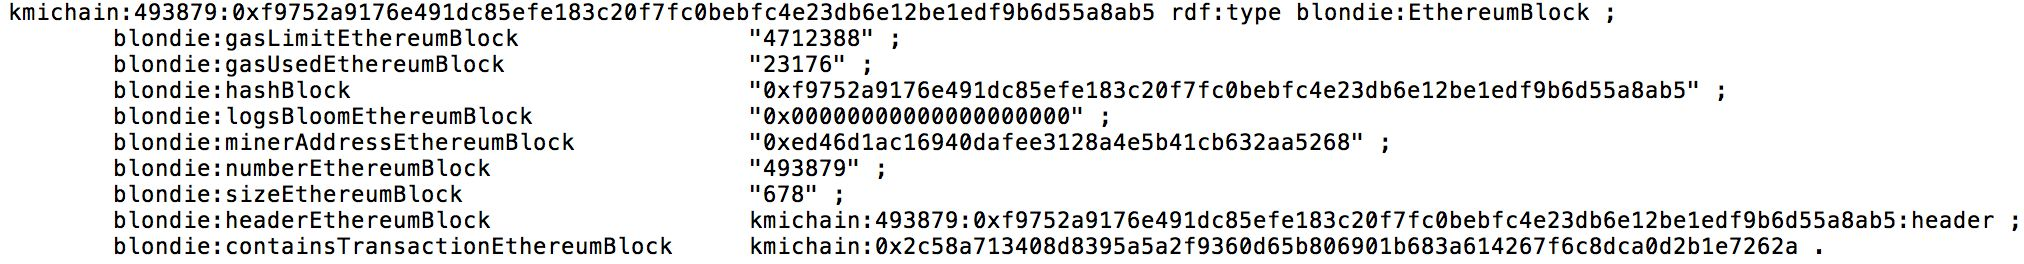
\includegraphics[width=1\textwidth]{resources/chapter-2/rdf-block.jpg}
  \caption{RDF dari deskripsi blok \parencite{third2017linked}}
  \label{image:rdf-block}
\end{figure}

\begin{figure}[ht]
  \centering
  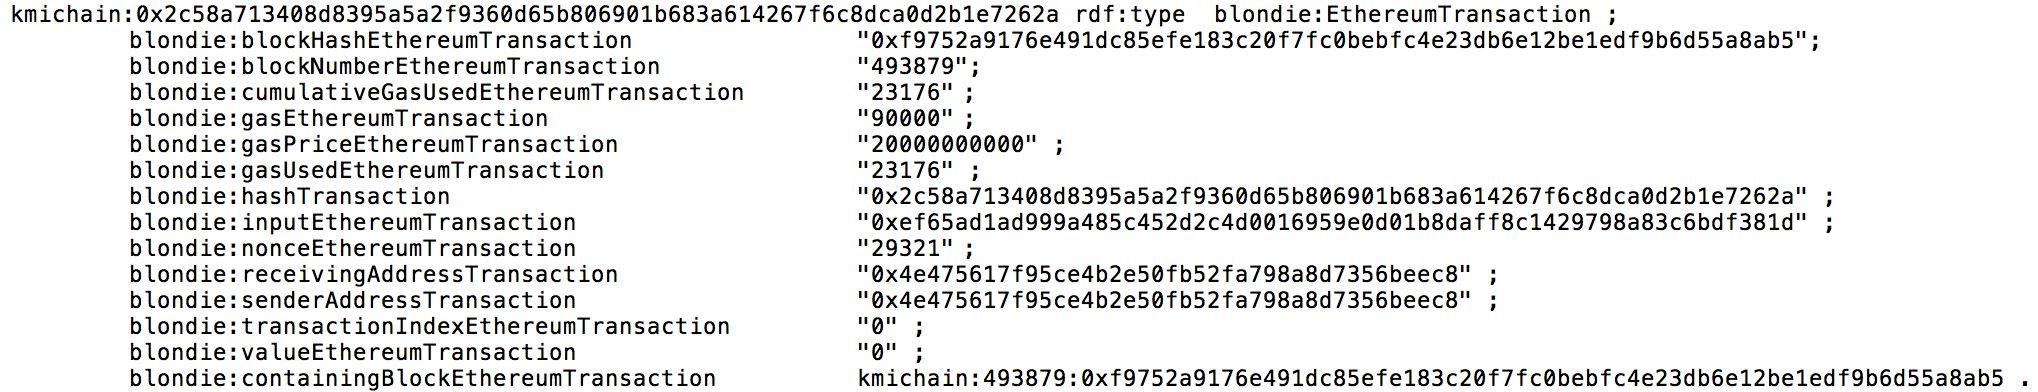
\includegraphics[width=1\textwidth]{resources/chapter-2/rdf-transaction.jpg}
  \caption{RDF dari deskripsi transaksi \parencite{third2017linked}}
  \label{image:rdf-transaction}
\end{figure}

Proyek ini diimplementasikan pada jaringan Ethereum Blockchain privat, di mana komponen \textit{listener} dikembangkan untuk mendeteksi blok baru dan mengindeksnya berdasarkan ontologi BLONDiE. RDF \textit{triples} kemudian dihasilkan dari data ini, yang memungkinkan penguraian data Blockchain secara semantik untuk mendukung pencarian data yang lebih terstruktur. Gambar \ref{image:rdf-block} dan gambar \ref{image:rdf-transaction} adalah contoh dari RDF \textit{triples} yang dihasilkan dari deskripsi blok dan transaksi masing-masing.

Hasil dari penelitian ini menunjukkan bahwa \textit{semantic indexing} memungkinkan data di dalam Blockchain menjadi lebih mudah diakses dan dapat terintegrasi dengan sumber data eksternal. Hal ini membuka peluang untuk mengembangkan \textit{semantic indexing} pada platform Blockchain lainnya serta berpotensi memperluas interoperabilitas data antara Blockchain dan \textit{Semantic Web}.